\documentclass[user_manual.tex]{subfiles}
\begin{document}
 \chapter{Nodos de ROS}
 
 %/////////////////////////////////////////////////////////////////////////////////////
%/////////////////////////////////////////////////////////////////////////////////////
\section{Hardware}
Sólo los nodos de esta carpeta interactúan con hardware. Todos los demás nodos sólo usan tópicos y servicios para obtener información del hardware.

%*************************************************************************************
%*************************************************************************************
\subsection{Head}

Dentro del paquete \texttt{head} se encuentra el nodo \texttt{head\_node.py}, este nodo se encarga de controlar la posición de la cabeza mediante los grados de libertad \textit{pan} y \textit{tilt}. La posición deseada se establece en radianes, en caso de que estos valores se encuentren fuera del rango de alcance de la articulación, entonces  se posicionará en la cota superior o inferior según sea el caso. En modo de simulación existe un nodo llamado \texttt{head\_simul\_node.py}, dicho nodo publica y se suscribe a los mismos tópicos.

%Principio de la tabla
\begin{table}[H]
\begin{center}
\begin{tabular}{|l|p{7cm}|p{4.5cm}|}%Define el número de columnas
\hline

\multirow{4}{*}{Tópicos publicados} 
&  /hardware/head/current\_pose [std\_msgs/Float32MultiArray]  & Posición actual de las juntas de la cabeza \\
& & \\
%& /tf (tf/tfMessage)  & Description\\
%& & \\
& /joint\_states [sensor\_msgs/JointState] & Descripción del estado de las juntas de la cabeza \\
& & \\
& /hardware/robot\_state/head\_battery [std\_msgs/Float32]  & Voltaje de alimentación de los servo motores de la cabeza\\ 
& & \\
\cline{1-3}

Tópicos suscritos &  /hardware/head/goal\_pose [std\_msgs/Float32MultiArray] & Posición deseada de las juntas de revolución de la cabeza \\ 
& & \\
\hline

\end{tabular}
\caption{Nodo /hardware/head}
\label{head node}
\end{center}
\end{table}
%Fin de la tabla

\textbf{Sintaxis en un archivo launch}

Para correr este nodo es necesario indicar como argumentos el puerto serial en el cual esta conectado el dispositivo \textit{USB2Dynamixel} asociado a los servo motores de la cabeza, así como el baudaje al cual se establecerá la comunicación.\\
\begin{minted}[
frame=lines,
framesep=1mm,
baselinestretch=1.2
]{xml}
<node name="head" pkg="head" type="head_node.py" output="screen" args="--port 
/dev/justinaHead --baud 1000000"/>
\end{minted}

%*************************************************************************************
%*************************************************************************************
\subsection{Arms}
El paquete \texttt{arms} contiene los nodos encargados del control de posición de las articulaciones de los brazos, los nombres de los ejecutables son \texttt{left\_arm\_node.py} y, \texttt{right\_arm\_node.py}. Debido a que ambos nodos operan del mismo modo, únicamente se explicará el nodo \texttt{left\_arm\_node.py}, la diferencia radica en los nombres dados a los tópicos, por ejemplo, el tópico \textit{/hardware/left\_arm/current\_pose} se llama \textit{/hardware/right\_arm/current\_pose} para el caso del nodo correspondiente al brazo derecho.\\

El nodo \texttt{left\_arm\_node.py} se encarga de controlar la posición de los 7 grados de libertad del brazo izquierdo del robot Justina, de igual modo controla el agarre del \textit{gripper}; la posición deseada para cada uno de los GDL se establece en radianes. Para el caso de simulación se encuentran los nodos \texttt{right\_arm\_simul\_node.py} y \texttt{left\_arm\_simul\_node.py}, los cuales funcionan de manera simular a los nodos de puesta en marcha del robot.

%Principio de la tabla
\begin{table}[H]
\begin{center}
\begin{tabular}{|l|p{7cm}|p{4.5cm}|}%Define el número de columnas
\hline

\multirow{5}{*}{Tópicos publicados}
& /hardware/left\_arm/current\_pose [std\_msgs/Float32MultiArray] & Posición actual de las juntas del brazo izquierdo \\
& & \\
& /hardware/left\_arm/current\_gripper [std\_msgs/Float32] & Posición actual del gripper \\
& & \\
%& /tf (tf/tfMessage) &  \\
%& & \\
& /joint\_states [sensor\_msgs/JointState] & Descripción del estado de las juntas del brazo izquierdo \\
& & \\
& /hardware/robot\_state/left\_arm\_battery [std\_msgs/Float32] & Voltaje de alimentación de los servo motores del brazo izquierdo \\
& & \\
\cline{1-3}

\multirow{3}{*}{Tópicos suscritos}
& /hardware/left\_arm/goal\_gripper [std\_msgs/Float32] & Posición deseada del gripper \\
& & \\
& /hardware/left\_arm/torque\_gripper [std\_msgs/Float32] & Par deseado en el gripper para tareas de manipulación de objetos \\
& & \\
& /hardware/left\_arm/goal\_pose [std\_msgs/Float32MultiArray] & Posición deseada de las juntas de revolución del brazo izquierdo. Si se especifican 7 datos, éstos serán las posiciones deseadas de los 7 GDL, si son 14 datos, los 7 adicionales serán las rapideces de los servo motores a las que se desea alcanzar dicha posición \\
& & \\
\cline{1-3}

\end{tabular}
\caption{Nodo /hardware/left\_arm}
\label{left arm node}
\end{center}
\end{table}
%Fin de la tabla

\textbf{Sintaxis en un archivo launch}\\
Para correr el nodo \texttt{left\_arm\_node.py} es necesario indicar como argumentos el puerto serial en el cual esta conectado el dispositivo \textit{USB2Dynamixel} asociado a los servo motores del brazo izquierdo, además del baudaje al cual se establecerá la comunicación.\\
\begin{minted}[
frame=lines,
framesep=1mm,
baselinestretch=1.2
]{xml}
<node name="left_arm" pkg="arms" type="left_arm_node.py" output="screen" args="--port1 
/dev/justinaLeftArm --baud1 1000000"/>
\end{minted}

%*************************************************************************************
%*************************************************************************************
\subsection{Mobile base}
En el paquete \texttt{mobile\_base} se encuentra el nodo \texttt{omni\_base\_node.py}, este nodo se encarga de controlar el movimiento de la base estableciendo la rapidez deseada para los motores por medio de controladores \textit{RoboClaw}, la velocidad y rapidez lineal están dadas en metros por segundo y, la velocidad angular en radianes por segundo. Además de esto, se determina la ubicación del robot en un mapa estático utilizando \textit{tf} y un mensaje de tipo \textit{Odometry}, para obtener información más detallada consulte por favor: \url{http://wiki.ros.org/navigation/Tutorials/RobotSetup/Odom}.
%Principio de la tabla
\begin{table}[H]
\begin{center}
\begin{tabular}{|l|p{6.5cm}|p{5.5cm}|}%Define el número de columnas
\hline

\multirow{3}{*}{Tópicos publicados}
& /hardware/mobile\_base/odometry [nav\_msgs/Odometry] & Odometría calculada con las lecturas de los encoder de los motores\\
& & \\
& /hardware/robot\_state/base\_battery [std\_msgs/Float32] & Voltaje de alimentación de los motores de la base \\
& & \\
& /tf [tf/tfMessage] & Transformación de \textit{base-link} a \textit{odom} \\
& & \\
\cline{1-3}

\multirow{3}{*}{Tópicos suscritos}
& /hardware/robot\_state/stop [std\_msgs/Empty] & Tópico para parar los motores de la base \\
& & \\
& /hardware/mobile\_base/cmd\_vel [geometry\_msgs/Twist] & Velocidad lineal deseada de la base en el plano \textit{xy}, y velocidad angular deseada de la base en el eje \textit{z} \\
& & \\
& /hardware/mobile\_base/speeds [std\_msgs/Float32MultiArray] & Rapideces instantáneas deseadas para las ruedas derecha e izquierda \\
& & \\
\cline{1-3}

\end{tabular}
\caption{Nodo /hardware/mobile\_base}
\label{mobile base node}
\end{center}
\end{table}
%Fin de la tabla

\textbf{Sintaxis en un archivo launch}

La base móvil con la que cuenta el robot Justina actualmente posee cuatro motores, es por ello que se requieren dos controladores \textit{RoboClaw}. Para lanzar este nodo se especifica mediante argumentos los dos puertos en los cuales están conectados los controladores.\\
\begin{minted}[
frame=lines,
framesep=1mm,
baselinestretch=1.2
]{xml}
<node name="mobile_base" pkg="mobile_base" type="omni_base_node.py" output="screen" 
args="--port1 /dev/justinaRC15 --port2 /dev/justinaRC30"/>
\end{minted}

%*************************************************************************************
%*************************************************************************************
\subsection{Laser simulator}

%*************************************************************************************
%*************************************************************************************
\subsection{Torso}

%Principio de la tabla
\begin{table}[H]
\begin{center}
\begin{tabular}{|l|p{6cm}|p{5cm}|}%Define el número de columnas
\hline

\multirow{4}{*}{Tópicos publicados}
& /hardware/torso/goal\_reached [std\_msgs/Bool] &  \\
& & \\
& /tf [tf/tfMessage] &  \\
& & \\
& /joint\_states \newline[sensor\_msgs/JointState] &  \\
& & \\
& /hardware/torso/current\_pose [std\_msgs/Float32MultiArray] &  \\
& & \\
\cline{1-3}

\multirow{2}{*}{Tópicos suscritos}
& /hardware/torso/goal\_pose [std\_msgs/Float32MultiArray] &  \\
& & \\
& /hardware/torso/goal\_rel\_pose [std\_msgs/Float32MultiArray] &  \\
& & \\
\cline{1-3} 

\end{tabular}
\caption{Nodo /hardware/torso}
\label{torso node}
\end{center}
\end{table}
%Fin de la tabla


%*************************************************************************************
%*************************************************************************************
%\subsection{Point Cloud Manager}

%*************************************************************************************
%*************************************************************************************
\subsection{Descripción del robot: URDF}
head\_pan        head\_node head\_simul\_node

head\_tilt.\\

En el archivo \textit{justina.xml} se encuentra el modelo del robot Justina; en la Figura   \ref{fig:URDF:Arbol} se tiene el árbol de transformaciones, los ovalos azules representan las juntas, mientras que los recuadros negros representan los sistemas de referencia asociados a los eslabones del robot. En el grafo dirigido se muestran los offset de traslación en \textit{x}, \textit{y} y \textit{z}, y los offset de los ángulos de rotación \textit{roll}, \textit{pitch} y \textit{yaw} que se tienen entre los sistemas de referencia, las unidades están en metros y radianes respectivamente.\\

En el grafo dirigido de la Figura \ref{fig:URDF:Frames} se muestran todas las transformaciones entre sistemas de referencia para el robot, en éste grafo se incluyen además los marcos \textit{odom} y \textit{map}. Para más información acerca de los sistemas de referencia para plataformas móviles consulte: \url{http://www.ros.org/reps/rep-0105.html}.

\begin{figure}[H]
\begin{center}
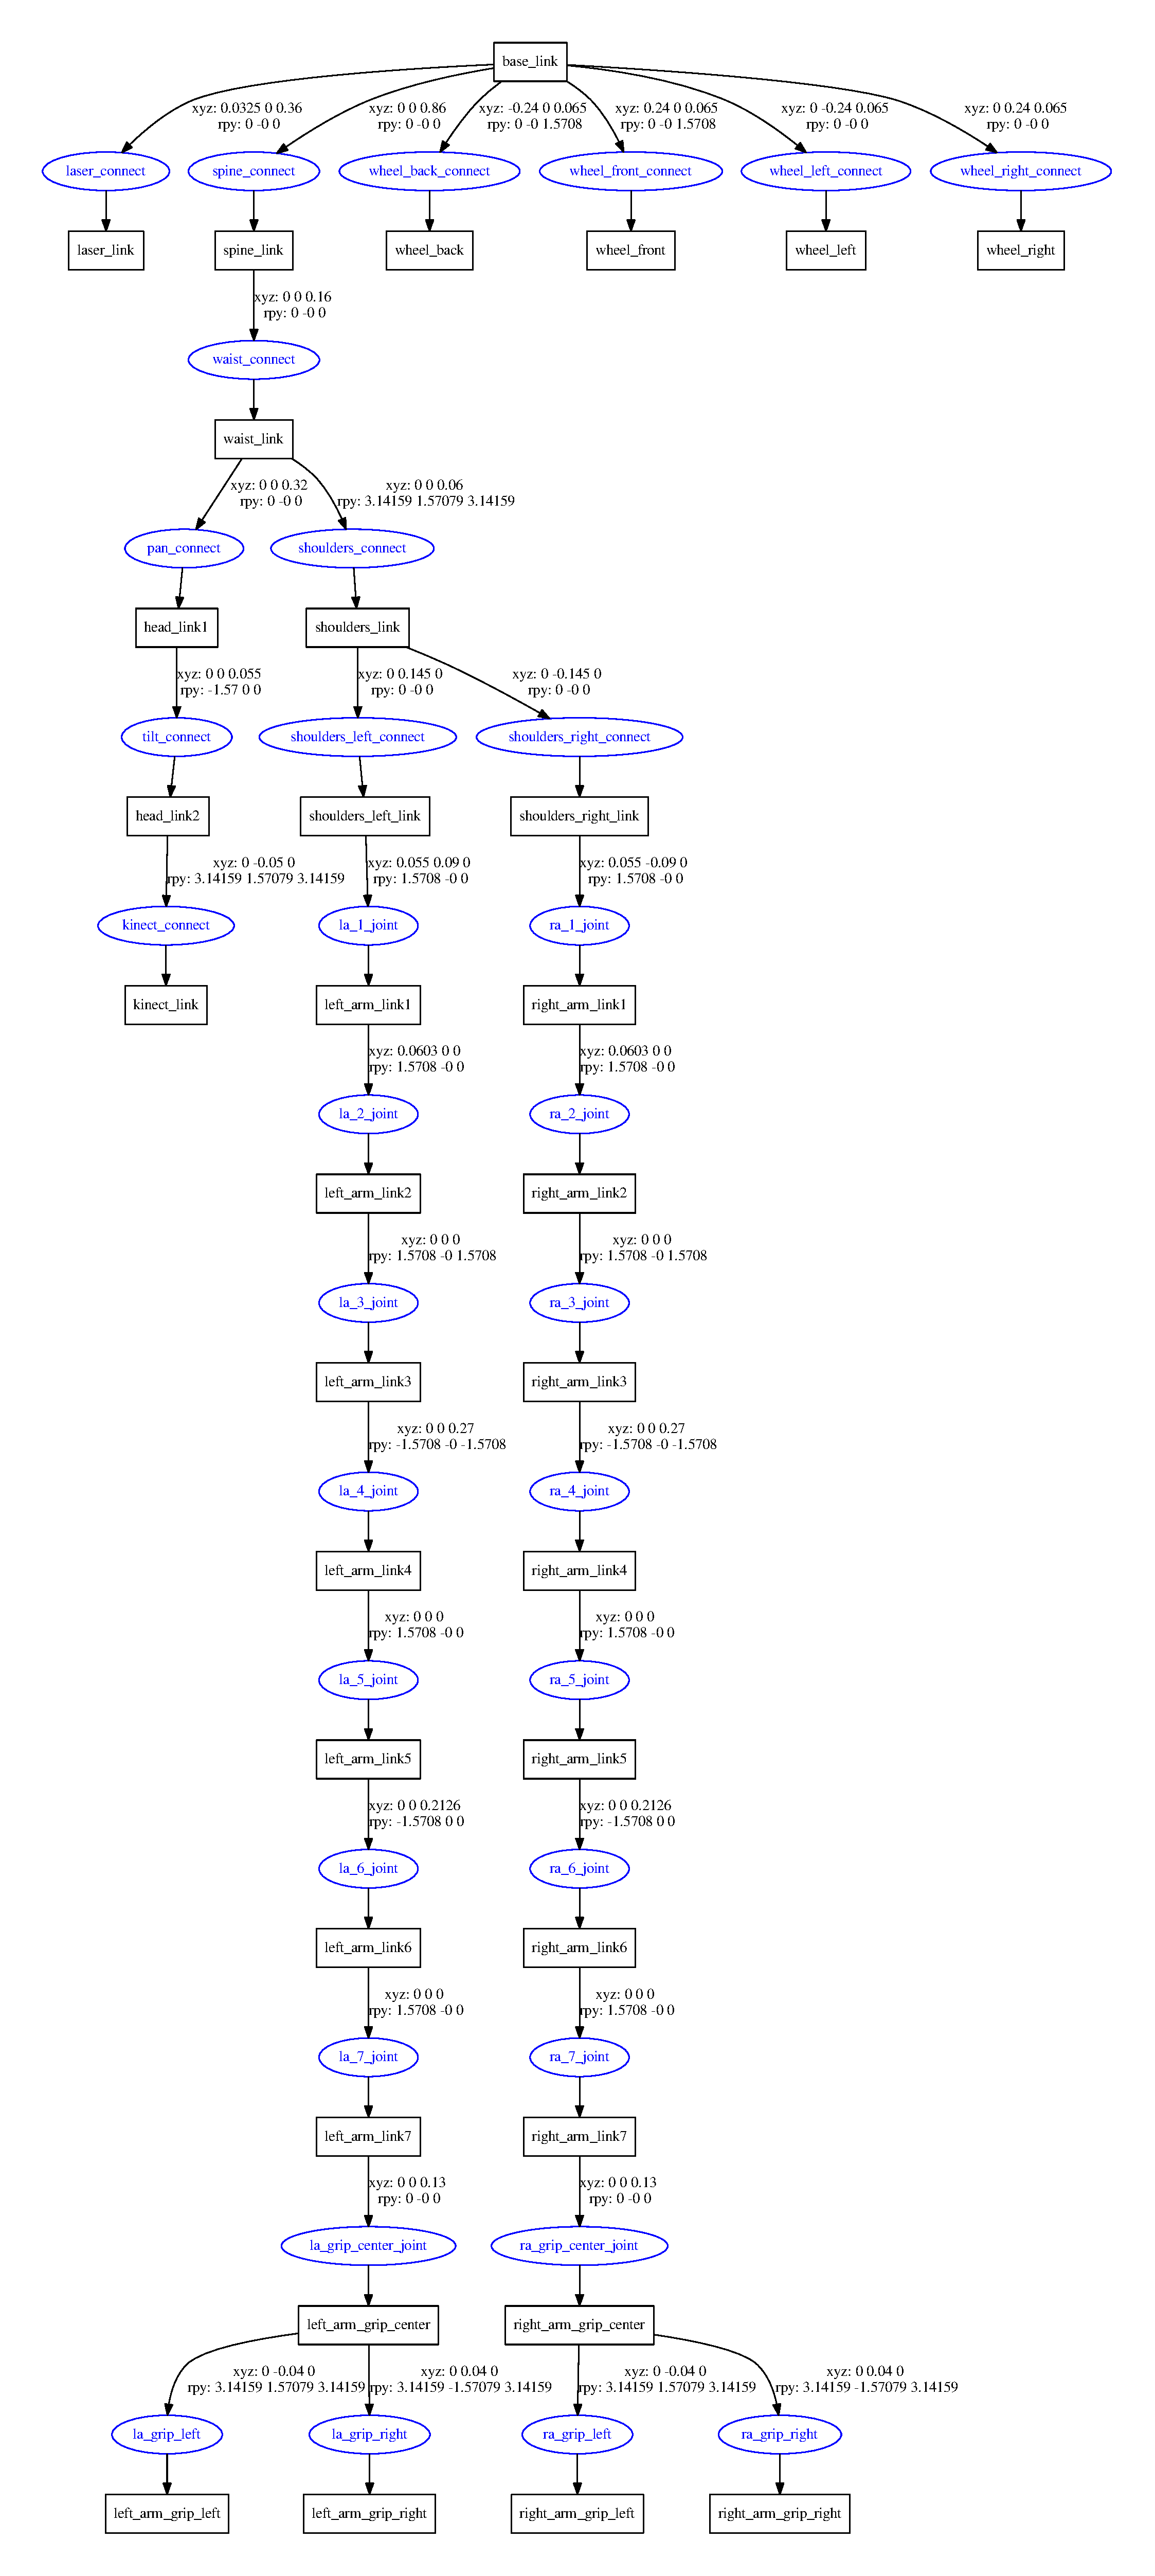
\includegraphics[scale=0.21]{Figures/Software/kinematic_tree/justina.pdf}
\end{center}
\caption{Árbol de transformaciones}
\label{fig:URDF:Arbol}
\end{figure}

\begin{figure}[H]
\begin{center}
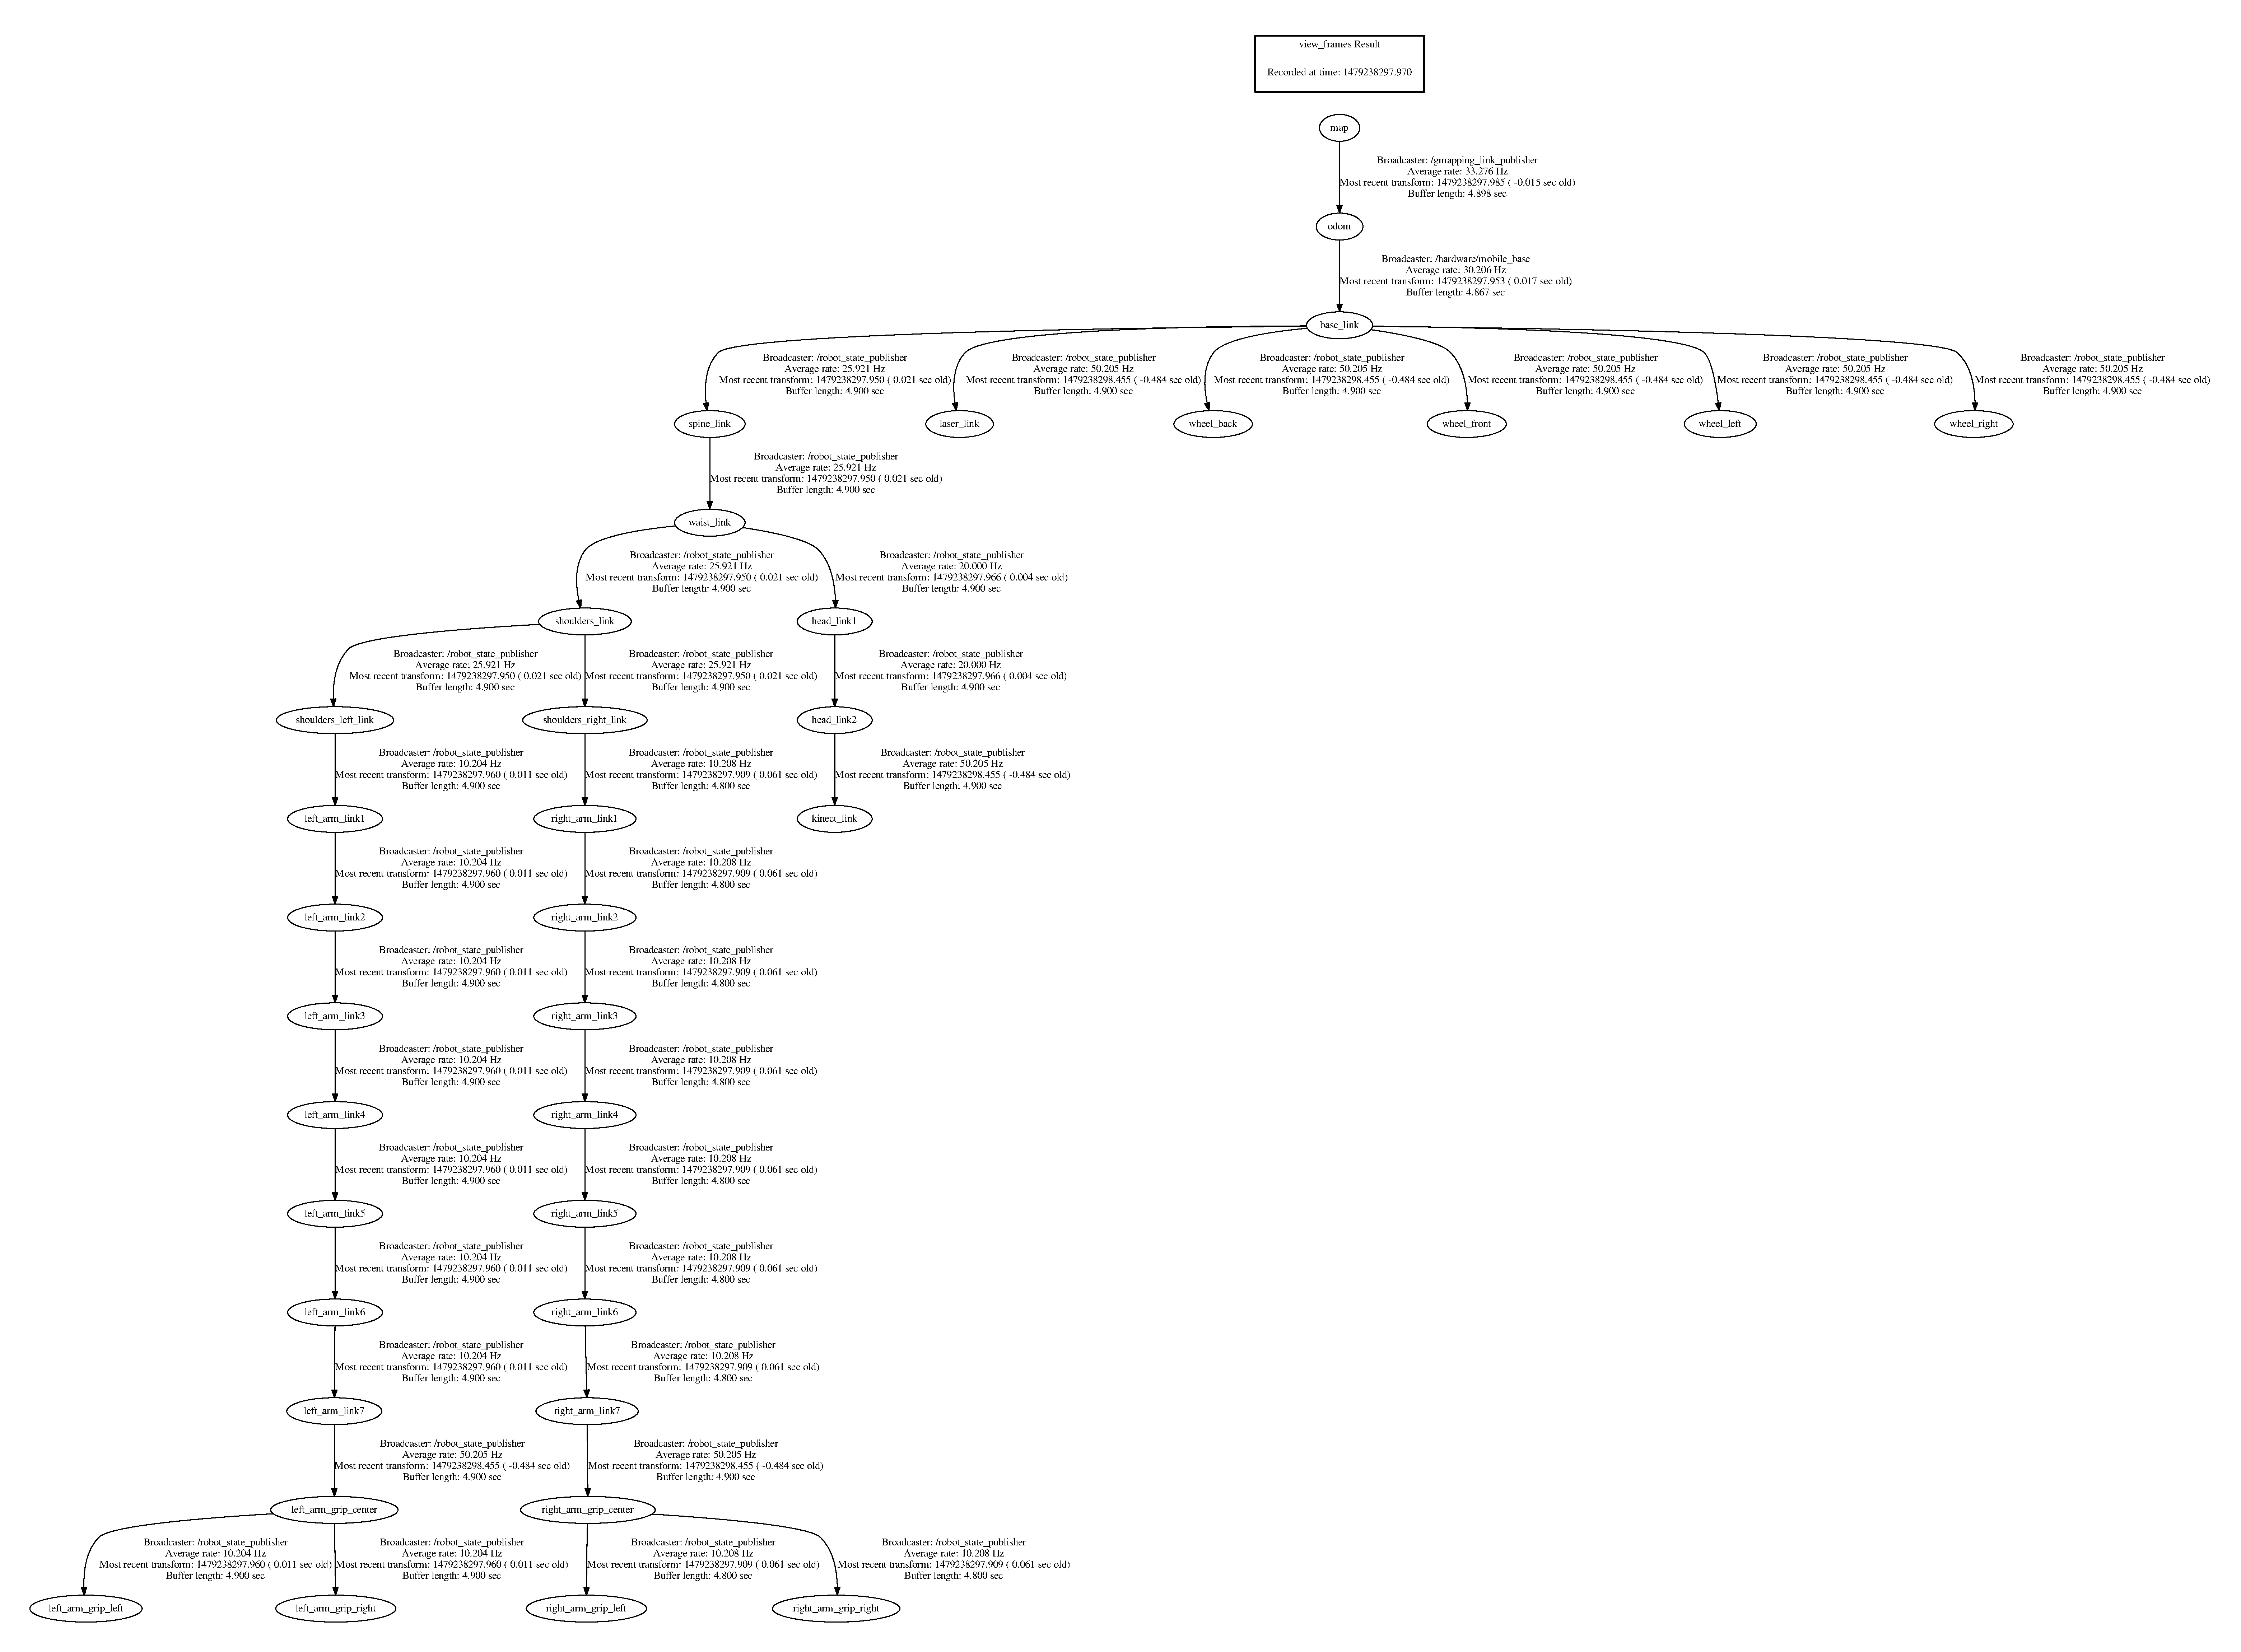
\includegraphics[scale=0.2, angle=90]{Figures/Software/kinematic_tree/frames.pdf}
\end{center}
\caption{Árbol de transformaciones con los marcos de referencia \textit{map} y \textit{odom}}
\label{fig:URDF:Frames}
\end{figure}

%/////////////////////////////////////////////////////////////////////////////////////
%/////////////////////////////////////////////////////////////////////////////////////
\section{Navigation}

%*************************************************************************************
%*************************************************************************************
\subsection{Obstacle detector}

%Principio de la tabla
\begin{table}[H]
\begin{center}
\begin{tabular}{|l|p{6.5cm}|p{5cm}|}%Define el número de columnas
\hline

\multirow{3}{*}{Tópicos publicados}
& /navigation/obs\_avoid/obs\_in\_front [std\_msgs/Bool] &  \\
& & \\
& /navigation/obs\_avoid/collision\_risk [std\_msgs/Bool] &  \\
& & \\
& /navigation/obs\_avoid/collision\_point [geometry\_msgs/PointStamped]  &  \\
& & \\
\cline{1-3}

\multirow{5}{*}{Tópicos suscritos}
& /hardware/scan \newline [sensor\_msgs/LaserScan] &  \\
& & \\
& /navigation/obs\_avoid/enable [std\_msgs/Bool]  &  \\
& & \\
& /tf [tf/tfMessage]  &  \\
& & \\
& /tf\_static [tf2\_msgs/TFMessage] &  \\
& & \\
& /navigation/mvn\_pln/last\_calc\_path [nav\_msgs/Path] &  \\
& & \\
\cline{1-3}
  
\end{tabular}
\caption{Nodo /navigation/obs\_avoid/obstacle\_detector}
\label{obs avoid obstacle detector node}
\end{center}
\end{table}
%Fin de la tabla

%*************************************************************************************
%*************************************************************************************
\subsection{Mvn Planner}
 
%Principio de la tabla
\begin{table}[H]
\begin{center}
\begin{tabular}{|l|p{7.2cm}|p{5cm}|}%Define el número de columnas
\hline

\multirow{9}{*}{Tópicos publicados}
& /navigation/path\_planning/simple\_move \newline /goal\_lateral [std\_msgs/Float32] &  \\
& & \\
& /hardware/torso/goal\_pose [std\_msgs/Float32MultiArray] &  \\
& & \\
& /manipulation/manip\_pln/hd\_goto\_loc [std\_msgs/String] &  \\
& & \\
& /manipulation/manip\_pln/ra\_goto\_loc [std\_msgs/String] &  \\
& & \\
& /hri/rviz/location\_markers \newline [visualization\_msgs/Marker] &  \\
& & \\
& /manipulation/manip\_pln/ \newline la\_goto\_angles [std\_msgs/Float32MultiArray] &  \\
& & \\
& /manipulation/manip\_pln/ \newline la\_pose\_wrt\_robot [std\_msgs/Float32MultiArray] &  \\
& & \\
& /navigation/path\_planning/simple\_move \newline /goal\_dist [std\_msgs/Float32] &  \\
& & \\
& /manipulation/manip\_pln/ \newline ra\_pose\_wrt\_robot [std\_msgs/Float32MultiArray] &  \\
& & \\
\cline{1-3}

\end{tabular}
\caption{Nodo /navigation/mvn\_pln}
\label{mvn pln node t1}
\end{center}
\end{table}
%Fin de la tabla

%Principio de la tabla
\begin{table}[H]
\begin{center}
\begin{tabular}{|l|p{7.1cm}|p{5cm}|}%Define el número de columnas
\hline

\multirow{9}{*}{Tópicos publicados}
& /navigation/mvn\_pln/get\_close\_xya [std\_msgs/Float32MultiArray] &  \\
& & \\
& /manipulation/manip\_pln/la\_move [std\_msgs/String] &  \\
& & \\
& /navigation/mvn\_pln/get\_close\_loc [std\_msgs/String] &  \\
& & \\
& /hardware/left\_arm/goal\_gripper [std\_msgs/Float32] &  \\
& & \\
& /navigation/path\_planning/simple\_move \newline /goal\_rel\_pose \newline [geometry\_msgs/Pose2D] &  \\
& & \\
& /hardware/right\_arm/torque\_gripper [std\_msgs/Float32] &  \\
& & \\
& /hardware/torso/goal\_rel\_pose [std\_msgs/Float32MultiArray] &  \\
& & \\
& /navigation/obs\_avoid/enable [std\_msgs/Bool] &  \\
& & \\
& /manipulation/manip\_pln/ \newline hd\_goto\_angles [std\_msgs/Float32MultiArray] &  \\
& & \\
\cline{1-3}

\end{tabular}
\caption{Nodo /navigation/mvn\_pln}
\label{mvn pln node t2}
\end{center}
\end{table}
%Fin de la tabla



%Principio de la tabla
\begin{table}[H]
\begin{center}
\begin{tabular}{|l|p{7.1cm}|p{5cm}|}%Define el número de columnas
\hline

\multirow{9}{*}{Tópicos publicados}
& /hardware/left\_arm/torque\_gripper [std\_msgs/Float32] &  \\
& & \\
& /navigation/path\_planning/simple\_move \newline /goal\_dist\_angle [std\_msgs/Float32MultiArray] &  \\
& & \\
& /manipulation/manip\_pln/ \newline la\_pose\_wrt\_arm [std\_msgs/Float32MultiArray] &  \\
& & \\
& /navigation/mvn\_pln/add\_location \newline [navig\_msgs/Location] &  \\
& & \\
& /navigation/mvn\_pln/last\_calc\_path [nav\_msgs/Path] &  \\
& & \\
& /navigation/global\_goal\_reached [std\_msgs/Bool] &  \\
& & \\
& /manipulation/manip\_pln/la\_goto\_loc [std\_msgs/String] &  \\
& & \\
& /navigation/path\_planning/simple\_move \newline /goal\_path [nav\_msgs/Path] &  \\
& & \\
& /navigation/path\_planning/simple\_move \newline /goal\_pose [geometry\_msgs/Pose2D] &  \\
& & \\
\cline{1-3}
  
\end{tabular}
\caption{Nodo /navigation/mvn\_pln}
\label{mvn pln node t3}
\end{center}
\end{table}
%Fin de la tabla

%Principio de la tabla
\begin{table}[H]
\begin{center}
\begin{tabular}{|l|p{6cm}|p{5cm}|}%Define el número de columnas
\hline

\multirow{3}{*}{Tópicos publicados}
& /manipulation/manip\_pln/ \newline ra\_goto\_angles [std\_msgs/Float32MultiArray] &  \\
& & \\
& /hardware/right\_arm/goal\_gripper [std\_msgs/Float32] &  \\
& & \\
& /manipulation/manip\_pln/ \newline ra\_pose\_wrt\_arm [std\_msgs/Float32MultiArray] &  \\
& & \\
\cline{1-3}

Servicios
& /navigation/mvn\_pln/plan\_path  &  \\
& & \\
\hline

\end{tabular}
\caption{Nodo /navigation/mvn\_pln}
\label{mvn pln node t4}
\end{center}
\end{table}
%Fin de la tabla

%Principio de la tabla
\begin{table}[H]
\begin{center}
\begin{tabular}{|l|p{6cm}|p{5cm}|}%Define el número de columnas
\hline

\multirow{9}{*}{Tópicos suscritos}
& /hardware/robot\_state/stop [std\_msgs/Empty] &  \\
& & \\
& /navigation/mvn\_pln/get\_close\_xya [std\_msgs/Float32MultiArray] &  \\
& & \\
& /clicked\_point \newline [geometry\_msgs/PointStamped] &  \\
& & \\
& /navigation/mvn\_pln/get\_close\_loc [std\_msgs/String] &  \\
& & \\
& /navigation/localization/current\_pose [geometry\_msgs/ \newline PoseWithCovarianceStamped] &  \\
& & \\
& /hardware/scan \newline [sensor\_msgs/LaserScan] &  \\
& & \\
& /hardware/torso/goal\_reached [std\_msgs/Bool] &  \\
& & \\
& /tf [tf/tfMessage]  &  \\
& & \\
& /navigation/obs\_avoid/obs\_in\_front [std\_msgs/Bool] &  \\
& & \\
\cline{1-3}

\end{tabular}
\caption{Nodo /navigation/mvn\_pln}
\label{mvn pln node t5}
\end{center}
\end{table}
%Fin de la tabla

%Principio de la tabla
\begin{table}[H]
\begin{center}
\begin{tabular}{|l|p{7cm}|p{5cm}|}%Define el número de columnas
\hline

\multirow{9}{*}{Tópicos suscritos}
& /tf\_static [tf2\_msgs/TFMessage]  &  \\
& & \\
& /manipulation/hd\_goal\_reached [std\_msgs/Bool] &  \\
& & \\
& /navigation/mvn\_pln/add\_location \newline [navig\_msgs/Location] &  \\
& & \\
& /manipulation/ra\_goal\_reached [std\_msgs/Bool] &  \\
& & \\
& /navigation/global\_goal\_reached [std\_msgs/Bool] &  \\
& & \\
& /navigation/obs\_avoid/collision\_risk [std\_msgs/Bool]  &  \\
& & \\
& /navigation/goal\_reached [std\_msgs/Bool] &  \\
& & \\
& /navigation/obs\_avoid/collision\_point [geometry\_msgs/PointStamped] &  \\
& & \\
& /manipulation/la\_goal\_reached [std\_msgs/Bool] &  \\
& & \\
\cline{1-3}

\end{tabular}
\caption{Nodo /navigation/mvn\_pln}
\label{mvn pln node t6}
\end{center}
\end{table}
%Fin de la tabla

%/////////////////////////////////////////////////////////////////////////////////////
%/////////////////////////////////////////////////////////////////////////////////////
\section{Vision}

%*************************************************************************************
%*************************************************************************************
\subsection{Face recognition}

%Principio de la tabla
\begin{table}[H]
\begin{center}
\begin{tabular}{|l|p{7.1cm}|p{5cm}|}%Define el número de columnas
\hline

\multirow{2}{*}{Tópicos publicados}
& /vision/face\_recognizer/faces \newline [vision\_msgs/VisionFaceObjects] &  \\
& & \\
& /vision/face\_recognizer/trainer\_result [std\_msgs/Int32] &  \\
& & \\
\cline{1-3}

\multirow{5}{*}{Tópicos suscritos}
& /vision/face\_recognizer/start\_recog\_old [std\_msgs/Empty]  &  \\
& & \\
& /vision/face\_recognizer/ \newline run\_face\_recognizer\_id [std\_msgs/String] &  \\
& & \\
& /vision/face\_recognizer/ \newline run\_face\_trainer\_frames \newline [vision\_msgs/VisionFaceTrainObject] &  \\
& & \\
& /vision/face\_recognizer/clearfacesdb [std\_msgs/Empty] &  \\
& & \\
& /vision/face\_recognizer/clearfacesdbbyid [std\_msgs/String] &  \\
& & \\
\cline{1-3}

\end{tabular}
\caption{Nodo /vision/face\_recog}
\label{face recog node t1}
\end{center}
\end{table}
%Fin de la tabla

%Principio de la tabla
\begin{table}[H]
\begin{center}
\begin{tabular}{|l|p{7.1cm}|p{5cm}|}%Define el número de columnas
\hline

\multirow{4}{*}{Tópicos suscritos}
& /vision/face\_recognizer/ \newline run\_face\_recognizer [std\_msgs/Empty] &  \\
& & \\
& /vision/face\_recognizer/run\_face\_trainer [std\_msgs/String] &  \\
& & \\
& /vision/face\_recognizer/stop\_recog [std\_msgs/Empty] &  \\
& & \\
& /vision/face\_recognizer/start\_recog [std\_msgs/Empty] &  \\
& & \\
\cline{1-3}

\end{tabular}
\caption{Nodo /vision/face\_recog}
\label{face recog node t2}
\end{center}
\end{table}
%Fin de la tabla

%*************************************************************************************
%*************************************************************************************
\subsection{Line finder}

%Principio de la tabla
\begin{table}[H]
\begin{center}
\begin{tabular}{|l|p{6.5cm}|p{5cm}|}%Define el número de columnas
\hline

Tópicos suscritos
& /hardware/head/current\_pose [std\_msgs/Float32MultiArray] &  \\
& & \\
\hline

Servicios
& /vision/line\_finder/find\_lines\_ransac [vision\_msgs/FindLines] &  \\
& & \\
\hline

\end{tabular}
\caption{Nodo /vision/line\_finder}
\label{line finder node}
\end{center}
\end{table}
%Fin de la tabla

%*************************************************************************************
%*************************************************************************************
\subsection{Object recognition}
El nodo se utiliza para detectar e identificar objetos sobre planos horizontales. Además, contiene las funciones para generar datos de entrenamiento que son utilizados durante el proceso de identificación. Actualmente, lo primero que se realiza para hacer la detección de objetos es una identificación y extracción de planos horizontales, para después segmentar la nube de puntos sobre estos planos y así identificar y clusterizar los objetos. Todo el proceso descrito anteriormente se realiza utilizando solamente información 3D. Una vez segmentados los objetos, estos se tratan de identificar utilizando 3 características:
\begin{itemize}
\item Altura (distancia del punto mas alejado del plano al plano)
\item Forma (se obtienen momentos de Hu de la proyección de los puntos del objeto sobre el plano)
\item Color (Se comparan Histogramas en HSV)
\end{itemize}

Estas tres características pasan por una etapa de clasificación similar a un clasificador en cascada y se devuelve el nombre del objeto entrenado más semejante al detectado. Además de esto, calcula el centroide de los objetos utilizando simplemente la media de todos los puntos 3D que lo componen.\\


%Principio de la tabla
\begin{table}[H]
\begin{center}
\begin{tabular}{|l|p{5.6cm}|p{6cm}|}%Define el número de columnas
\hline

Tópicos publicados
& /vision/obj\_reco \newline /recognizedObjectes \newline [vision\_msgs/VisionObjectList] &  Si el tópico enableRecognizeTopic recibe el valor True en el callback, entonces el nodo detecta y trata de identificar todos los objetos que se encuentren sobre los planos horizontales utilizando los datos de entrenamiento previos, cada que hay un nuevo frame de Kinect. En el tópico se publican los nombres de los objetos identificados, así como las coordenadas de su centroide. \\
& & \\
\hline
 
\end{tabular}
\caption{Nodo /vision/obj\_reco}
\label{obj reco node t1}
\end{center}
\end{table}
%Fin de la tabla

%Principio de la tabla
\begin{table}[H]
\begin{center}
\begin{tabular}{|l|p{5.4cm}|p{6.5cm}|}%Define el número de columnas
\hline

Tópicos suscritos
& /vision/obj\_reco \newline /enableRecognizeTopic [std\_msgs/Bool] & Habilita o deshabilita la función de reconocimiento de objetos cada que existe un nuevo frame de Kinect. \\
& & \\
& /vision/obj\_reco \newline /enableDetectWindow [std\_msgs/Bool] & Habilita o deshabilita la ventana donde se muestra el reconocimiento de objetos cada que existe un nuevo frame de Kinect. Para evitar consumir recursos, se recomienda que esta este en false, salvo para depuración o entrenamiento. \\
& & \\
& /hardware/point\_cloud\_man/ \newline rgbd\_wrt\_robot \newline [sensor\_msgs/PointCloud2] & Si alguno de los dos tópicos anteriores esta habilitado, el nodo espera este tópico para realizar la detección e identificación de objetos con cada nuevo frame. \\
& & \\
\cline{1-3}
 
\end{tabular}
\caption{Nodo /vision/obj\_reco}
\label{obj reco node t2}
\end{center}
\end{table}
%Fin de la tabla

%Principio de la tabla
\begin{table}[H]
\begin{center}
\begin{tabular}{|l|p{5.3cm}|p{8cm}|}%Define el número de columnas
\hline

Servicios
& /vision/obj\_reco/det\_objs \newline [vision\_msgs/DetectObjects] & El nodo detecta el plano horizontal más grande en la escena, y detecta todos los objetos sobre este usando información 3D. Una vez detectados, estos objetos tratan de ser reconocidos utilizando las características extraídas durante la fase de entrenamiento. El servicio regresa una lista de todos los objetos \textbf{reconocidos}, utilizando su nombre y su centroide con respecto del robot.  \\
& & \\
& /vision/geometry\_finder /findPlane \newline [vision\_msgs/FindPlane] & Detecta y muestra en una ventana todos los planos \textbf{horizontales} detectados. \\
& & \\
& /vision/obj\_reco/trainObject [vision\_msgs/TrainObject] & Se le envía un string con el nombre de un objeto y el nodo detecta y extrae las características 3D y 2D del objeto más cercano al centro del robot (los objetos, para ser detectados, deben encontrarse sobre un plano horizontal). Un archivo XML con las características del objeto, nombre y una imagen del objeto es guardado en el directorio: \textbackslash src\textbackslash vision\textbackslash obj\_reco\textbackslash TrainingDir \textbackslash NombreDelObjeto\\
& & \\
\cline{1-3}
 
\end{tabular}
\caption{Nodo /vision/obj\_reco}
\label{obj reco node t3}
\end{center}
\end{table}
%Fin de la tabla

%*************************************************************************************
%*************************************************************************************
\subsection{Skeleton finder}

%Principio de la tabla
\begin{table}[H]
\begin{center}
\begin{tabular}{|l|p{6cm}|p{5cm}|}%Define el número de columnas
\hline

Tópicos publicados
& /vision/skeleton\_finder/skeletons \newline [vision\_msgs/Skeletons] &  \\
& & \\
\hline

\multirow{2}{*}{Tópicos suscritos}
& /vision/skeleton\_finder/start\_recog [std\_msgs/Empty] &  \\
& & \\
& /vision/skeleton\_finder/stop\_recog [std\_msgs/Empty] &  \\
& & \\
\cline{1-3}
 
\end{tabular}
\caption{Nodo /vision/skeleton\_finder}
\label{skeleton finder node}
\end{center}
\end{table}
%Fin de la tabla

%/////////////////////////////////////////////////////////////////////////////////////
%/////////////////////////////////////////////////////////////////////////////////////
\section{Human-robot interaction}

%*************************************************************************************
%*************************************************************************************
\subsection{gui}
Sirve para operar todo el robot desde una interfaz gráfica cuyas funciones se detallan en la sección \ref{sec:GUI}.

%Principio de la tabla
\begin{table}[H]
\begin{center}
\begin{tabular}{|l|p{7.1cm}|p{5cm}|}%Define el número de columnas
\hline

\multirow{4}{*}{Tópicos publicados}
& /hardware/point\_cloud\_man/save\_cloud [std\_msgs/String] &  \\
& & \\
& /navigation/path\_planning/ \newline simple\_move/goal\_lateral [std\_msgs/Float32] &  \\
& & \\
& /hardware/torso/goal\_pose [std\_msgs/Float32MultiArray] &  \\
& & \\
& /manipulation/manip\_pln/hd\_goto\_loc [std\_msgs/String] &  \\
& & \\
& /hardware/robot\_state/stop [std\_msgs/Empty] &  \\
& & \\
& /vision/face\_recognizer/start\_recog\_old [std\_msgs/Empty] &  \\
& & \\
& /manipulation/manip\_pln/ra\_goto\_loc [std\_msgs/String] &  \\
& & \\
& /manipulation/manip\_pln/ \newline la\_goto\_angles [std\_msgs/Float32MultiArray] &  \\
& & \\
& /manipulation/manip\_pln/ \newline la\_pose\_wrt\_robot [std\_msgs/Float32MultiArray] &  \\
& & \\
& /navigation/path\_planning/ \newline simple\_move/goal\_dist [std\_msgs/Float32] &  \\
& & \\

\cline{1-3}
\end{tabular}
\caption{Nodo /hri/justina\_gui}
\label{justina gui node t1}
\end{center}
\end{table}
%Fin de la tabla



%Principio de la tabla
\begin{table}[H]
\begin{center}
\begin{tabular}{|l|p{7cm}|p{5cm}|}%Define el número de columnas
\hline

\multirow{4}{*}{Tópicos publicados}
& /vision/face\_recognizer/ \newline run\_face\_recognizer\_id [std\_msgs/String] &  \\
& & \\
& /hardware/point\_cloud\_man/ \newline stop\_saving\_cloud [std\_msgs/Empty] &  \\
& & \\
& /hardware/mobile\_base/cmd\_vel \newline [geometry\_msgs/Twist] &  \\
& & \\
& /manipulation/manip\_pln/ \newline ra\_pose\_wrt\_robot [std\_msgs/Float32MultiArray] &  \\
& & \\
& /navigation/mvn\_pln/get\_close\_xya [std\_msgs/Float32MultiArray] &  \\
& & \\
& /hardware/right\_arm/goal\_torque [std\_msgs/Float32MultiArray] &  \\
& & \\
& /manipulation/manip\_pln/la\_move [std\_msgs/String] &  \\
& & \\
& /navigation/mvn\_pln/get\_close\_loc [std\_msgs/String] &  \\
& & \\
& /vision/obj\_reco/enableRecognizeTopic [std\_msgs/Bool] &  \\
& & \\
& /hardware/left\_arm/goal\_gripper [std\_msgs/Float32] &  \\
& & \\

\cline{1-3}
\end{tabular}
\caption{Nodo /hri/justina\_gui}
\label{justina gui node t2}
\end{center}
\end{table}
%Fin de la tabla



%Principio de la tabla
\begin{table}[H]
\begin{center}
\begin{tabular}{|l|p{7cm}|p{5cm}|}%Define el número de columnas
\hline

\multirow{4}{*}{Tópicos publicados}
& /hardware/mobile\_base/speeds [std\_msgs/Float32MultiArray] &  \\
& & \\
& /recognizedSpeech [hri\_msgs/RecognizedSpeech] &  \\
& & \\
& /hardware/head/goal\_pose [std\_msgs/Float32MultiArray] &  \\
& & \\
& /navigation/path\_planning/ \newline simple\_move/goal\_rel\_pose \newline [geometry\_msgs/Pose2D] &  \\
& & \\
& /hri/human\_following/start\_follow [std\_msgs/Bool] &  \\
& & \\
& /vision/obj\_reco/enableDetectWindow [std\_msgs/Bool] &  \\
& & \\
& /hardware/right\_arm/torque\_gripper [std\_msgs/Float32] &  \\
& & \\
& /vision/face\_recognizer/ \newline run\_face\_trainer\_frames \newline [vision\_msgs/VisionFaceTrainObject] &  \\
& & \\
& /hardware/torso/goal\_rel\_pose [std\_msgs/Float32MultiArray] &  \\
& & \\
& /navigation/obs\_avoid/enable [std\_msgs/Bool] &  \\
& & \\

\cline{1-3}
\end{tabular}
\caption{Nodo /hri/justina\_gui}
\label{justina gui node t3}
\end{center}
\end{table}
%Fin de la tabla





%Principio de la tabla
\begin{table}[H]
\begin{center}
\begin{tabular}{|l|p{7.1cm}|p{5cm}|}%Define el número de columnas
\hline

\multirow{4}{*}{Tópicos publicados}
& /vision/thermal\_vision/stop\_video [std\_msgs/Empty] &  \\
& & \\
& /vision/skeleton\_finder/stop\_recog [std\_msgs/Empty] &  \\
& & \\
& /vision/face\_recognizer/clearfacesdb [std\_msgs/Empty] &  \\
& & \\
& /manipulation/manip\_pln/ \newline hd\_goto\_angles [std\_msgs/Float32MultiArray] &  \\
& & \\
& /hardware/left\_arm/goal\_torque [std\_msgs/Float32MultiArray] &  \\
& & \\
& /vision/face\_recognizer/clearfacesdbbyid [std\_msgs/String] &  \\
& & \\
& /hardware/left\_arm/torque\_gripper [std\_msgs/Float32] &  \\
& & \\
& /navigation/path\_planning/ \newline simple\_move/goal\_dist\_angle [std\_msgs/Float32MultiArray] &  \\
& & \\
& /manipulation/manip\_pln/ \newline la\_pose\_wrt\_arm [std\_msgs/Float32MultiArray] &  \\
& & \\
& /hardware/left\_arm/goal\_pose [std\_msgs/Float32MultiArray] &  \\
& & \\

\cline{1-3}
\end{tabular}
\caption{Nodo /hri/justina\_gui}
\label{justina gui node t4}
\end{center}
\end{table}
%Fin de la tabla






%Principio de la tabla
\begin{table}[H]
\begin{center}
\begin{tabular}{|l|p{7.1cm}|p{5cm}|}%Define el número de columnas
\hline

\multirow{4}{*}{Tópicos publicados}
& /navigation/mvn\_pln/add\_location \newline [navig\_msgs/Location] &  \\
& & \\
& /hri/leg\_finder/enable [std\_msgs/Bool] &  \\
& & \\
& /vision/face\_recognizer/ \newline run\_face\_recognizer [std\_msgs/Empty] &  \\
& & \\
& /hri/sp\_rec/recognized [std\_msgs/String] &  \\
& & \\
& /vision/thermal\_vision/start\_video [std\_msgs/Empty] &  \\
& & \\
& /vision/face\_recognizer/run\_face\_trainer [std\_msgs/String] &  \\
& & \\
& /manipulation/manip\_pln/la\_goto\_loc [std\_msgs/String] &  \\
& & \\
& /vision/face\_recognizer/stop\_recog [std\_msgs/Empty] &  \\
& & \\
& /hardware/right\_arm/goal\_pose [std\_msgs/Float32MultiArray] &  \\
& & \\
& /vision/face\_recognizer/start\_recog [std\_msgs/Empty] &  \\
& & \\

\cline{1-3}
\end{tabular}
\caption{Nodo /hri/justina\_gui}
\label{justina gui node t5}
\end{center}
\end{table}
%Fin de la tabla




%Principio de la tabla
\begin{table}[H]
\begin{center}
\begin{tabular}{|l|p{7.1cm}|p{5cm}|}%Define el número de columnas
\hline

\multirow{4}{*}{Tópicos publicados}
& /navigation/path\_planning/simple\_move \newline /goal\_path [nav\_msgs/Path]  &  \\
& & \\
& /vision/skeleton\_finder/start\_recog [std\_msgs/Empty] &  \\
& & \\
& /navigation/path\_planning/simple\_move \newline /goal\_pose [geometry\_msgs/Pose2D] &  \\
& & \\
& /vision/qr/start\_qr [std\_msgs/Bool] &  \\
& & \\
& /manipulation/manip\_pln \newline /ra\_goto\_angles [std\_msgs/Float32MultiArray] &  \\
& & \\
& /hardware/right\_arm/goal\_gripper [std\_msgs/Float32] &  \\
& & \\
& /manipulation/manip\_pln \newline /ra\_pose\_wrt\_arm [std\_msgs/Float32MultiArray] &  \\
& & \\

\cline{1-3}
\end{tabular}
\caption{Nodo /hri/justina\_gui}
\label{justina gui node t6}
\end{center}
\end{table}
%Fin de la tabla






%Principio de la tabla
\begin{table}[H]
\begin{center}
\begin{tabular}{|l|p{7cm}|p{5cm}|}%Define el número de columnas
\hline

\multirow{4}{*}{Tópicos suscritos}
& /hardware/left\_arm/current\_pose [std\_msgs/Float32MultiArray] &  \\
& & \\
& /hardware/robot\_state/stop [std\_msgs/Empty] &  \\
& & \\
& /vision/face\_recognizer/faces \newline [vision\_msgs/VisionFaceObjects] &  \\
& & \\
& /recognizedSpeech [hri\_msgs/RecognizedSpeech] &  \\
& & \\
& /hardware/left\_arm/current\_gripper [std\_msgs/Float32] &  \\
& & \\
& /hri/leg\_finder/legs\_found [std\_msgs/Empty] &  \\
& & \\
& /hardware/right\_arm/current\_gripper [] &  \\
& & \\
& /navigation/localization/current\_pose [geometry\_msgs/ \newline PoseWithCovarianceStamped] &  \\
& & \\
& /hardware/head/current\_pose [std\_msgs/Float32MultiArray] &  \\
& & \\
& /hardware/torso/goal\_reached [std\_msgs/Bool] &  \\
& & \\


\cline{1-3}
\end{tabular}
\caption{Nodo /hri/justina\_gui}
\label{justina gui node t7}
\end{center}
\end{table}
%Fin de la tabla



%Principio de la tabla
\begin{table}[H]
\begin{center}
\begin{tabular}{|l|p{6.4cm}|p{5cm}|}%Define el número de columnas
\hline

\multirow{4}{*}{Tópicos suscritos}
& /tf [tf/tfMessage] &  \\
& & \\
& /navigation/obs\_avoid/obs\_in\_front [std\_msgs/Bool] &  \\
& & \\
& /tf\_static [tf2\_msgs/TFMessage] &  \\
& & \\
& /manipulation/hd\_goal\_reached [std\_msgs/Bool] &  \\
& & \\
& /hri/sp\_rec/recognized [std\_msgs/String] &  \\
& & \\
& /hardware/robot\_state/ \newline right\_arm\_battery [] &  \\
& & \\
& /hardware/right\_arm/current\_pose [] &  \\
& & \\
& /hardware/torso/current\_pose [std\_msgs/Float32MultiArray] &  \\
& & \\
& /manipulation/ra\_goal\_reached [std\_msgs/Bool] &  \\
& & \\
& /navigation/global\_goal\_reached [std\_msgs/Bool] &  \\
& & \\

\cline{1-3}
\end{tabular}
\caption{Nodo /hri/justina\_gui}
\label{justina gui node t8}
\end{center}
\end{table}
%Fin de la tabla





%Principio de la tabla
\begin{table}[H]
\begin{center}
\begin{tabular}{|l|p{7cm}|p{5cm}|}%Define el número de columnas
\hline

\multirow{4}{*}{Tópicos suscritos}
& /navigation/obs\_avoid/collision\_risk [std\_msgs/Bool] &  \\
& & \\
& /navigation/goal\_reached [std\_msgs/Bool] &  \\
& & \\
& /vision/face\_recognizer/trainer\_result [std\_msgs/Int32] &  \\
& & \\
& /hardware/robot\_state/left\_arm\_battery [std\_msgs/Float32] &  \\
& & \\
& /hardware/robot\_state/head\_battery [std\_msgs/Float32] &  \\
& & \\
& /hri/qr/recognized [std\_msgs/String] &  \\
& & \\
& /manipulation/la\_goal\_reached [std\_msgs/Bool] &  \\
& & \\
& /hardware/robot\_state/base\_battery [std\_msgs/Float32] &  \\
& & \\ 

\cline{1-3}
\end{tabular}
\caption{Nodo /hri/justina\_gui}
\label{justina gui node t9}
\end{center}
\end{table}
%Fin de la tabla

%*************************************************************************************
%*************************************************************************************
\subsection{Human follower}

%Principio de la tabla
\begin{table}[H]
\begin{center}
\begin{tabular}{|l|p{6cm}|p{5cm}|}%Define el número de columnas
\hline

Tópicos publicados
& /hardware/mobile\_base/speeds [std\_msgs/Float32MultiArray] &  \\
& & \\
\hline

\multirow{2}{*}{Tópicos suscritos}
& /hri/human\_following/start\_follow [std\_msgs/Bool] &  \\
& & \\
& /hri/leg\_finder/leg\_poses \newline[geometry\_msgs/PointStamped] &  \\
& & \\
\cline{1-3}

\end{tabular}
\caption{Nodo /hri/human\_follower}
\label{human follower node}
\end{center}
\end{table}
%Fin de la tabla

%*************************************************************************************
%*************************************************************************************
\subsection{Leg finder}

%Principio de la tabla
\begin{table}[H]
\begin{center}
\begin{tabular}{|l|p{6cm}|p{5cm}|}%Define el número de columnas
\hline

\multirow{2}{*}{Tópicos publicados}
& /hri/leg\_finder/legs\_found [std\_msgs/Empty] &  \\
& & \\
& /hri/leg\_finder/leg\_poses \newline [geometry\_msgs/PointStamped] &  \\
& & \\
\cline{1-3}

\multirow{4}{*}{Tópicos suscritos}
& /hardware/scan \newline [sensor\_msgs/LaserScan] &  \\
& & \\
& /tf [tf/tfMessage] &  \\
& & \\
& /tf\_static [tf2\_msgs/TFMessage] &  \\
& & \\
& /hri/leg\_finder/enable [std\_msgs/Bool]  &  \\
& & \\
\cline{1-3}

\end{tabular}
\caption{Nodo /hri/leg\_finder}
\label{leg finder node}
\end{center}
\end{table}
%Fin de la tabla

%*************************************************************************************
%*************************************************************************************
\subsection{QR reader}

%Principio de la tabla
\begin{table}[H]
\begin{center}
\begin{tabular}{|l|p{6cm}|p{5cm}|}%Define el número de columnas
\hline

Tópicos publicados
& /hri/qr/recognized [std\_msgs/String] &  \\
& & \\
\hline

\multirow{3}{*}{Tópicos suscritos}
& /tf [tf/tfMessage] &  \\
& & \\
& /tf\_static [tf2\_msgs/TFMessage] &  \\
& & \\
& /vision/qr/start\_qr [std\_msgs/Bool] &  \\
& & \\
\cline{1-3}

\end{tabular}
\caption{Nodo /hri/qr\_reader}
\label{qr reader node}
\end{center}
\end{table}
%Fin de la tabla

%*************************************************************************************
%*************************************************************************************
\subsection{SP gen}

%Principio de la tabla
\begin{table}[H]
\begin{center}
\begin{tabular}{|l|p{6cm}|p{5cm}|}%Define el número de columnas
\hline

Tópicos suscritos
& /hri/sp\_gen/say [std\_msgs/String] &  \\
& & \\
\hline

\end{tabular}
\caption{Nodo /hri/sp\_gen}
\label{sp gen node}
\end{center}
\end{table}
%Fin de la tabla

%/////////////////////////////////////////////////////////////////////////////////////
%/////////////////////////////////////////////////////////////////////////////////////
\section{Interoperation}

%*************************************************************************************
%*************************************************************************************
\subsection{Joystick teleop}
Este nodo se suscribe a un mensaje de tipo \textit{Joy} para controlar mediante un joystick de una consola Xbox el movimiento de la base, la posición de la cabeza y del torso. Las posiciones angulares y lineales, así como las velocidades lineales y angulares están dadas en radianes, metros, metros por segundo y radianes por segundo respectivamente.\\

Para mover la cabeza del robot se utiliza el \textit{stick} izquierdo, la base se opera por medio del \textit{stick} derecho, mientras que el botón rojo del joystick es para el paro de la base.\\

%Principio de la tabla
\begin{table}[H]
\begin{center}
\begin{tabular}{|l|p{6cm}|p{5cm}|}%Define el número de columnas
\hline

\multirow{6}{*}{Tópicos publicados}
& /hardware/robot\_state/stop [std\_msgs/Empty] & Tópico de paro para los motores de la base \\
& & \\
& /hardware/mobile\_base/cmd\_vel \newline [geometry\_msgs/Twist] & Velocidad lineal deseada deseada de la base en el plano \textit{xy}, y velocidad angular deseada en \textit{z} \\
& & \\
& /hardware/head/goal\_pose [std\_msgs/Float32MultiArray] & Posición deseada de la cabeza \\
& & \\
& /hardware/torso/goal\_spine [std\_msgs/Float32] & Posición deseada de la junta prismática para cambiar la altura del torso \\
& & \\
& /hardware/torso/goal\_shoulders [std\_msgs/Float32] & Posición deseada de la junta de revolución para orientar el torso (roll) \\
& & \\
& /hardware/torso/goal\_waist [std\_msgs/Float32] & Posición deseada de la junta de revolución para orientar el torso (yaw) \\
& & \\
\cline{1-3}

Tópicos suscritos
& /hardware/joy [sensor\_msgs/Joy]  & Estado de los ejes y botones de un joystick \\
& & \\
\hline

\end{tabular}
\caption{Nodo /interoperation/joystick\_teleop}
\label{joystick teleop node}
\end{center}
\end{table}
%Fin de la tabla

\textbf{Sintaxis en un archivo launch}

Para lanzar este nodo por medio de un archivo \textit{lauch} sólo se necesita indicar el nombre que se le desea dar al nodo, el paquete dentro del que se encuentra y el nombre del ejecutable.\\
\begin{minted}[
frame=lines,
framesep=1mm,
baselinestretch=1.2
]{xml}
<node name="joystick_teleop" pkg="joystick_teleop" type="joystick_teleop_node.py" 
output="screen" />
\end{minted}


%/////////////////////////////////////////////////////////////////////////////////////
%/////////////////////////////////////////////////////////////////////////////////////
\section{Manipulation}

%*************************************************************************************
%*************************************************************************************
\subsection{Manipulation Planner}

%Principio de la tabla
\begin{table}[H]
\begin{center}
\begin{tabular}{|l|p{6cm}|p{5cm}|}%Define el número de columnas
\hline

\multirow{9}{*}{Tópicos publicados}
& /hardware/right\_arm/goal\_torque [std\_msgs/Float32MultiArray] &  \\
& & \\
& /hardware/head/goal\_pose [std\_msgs/Float32MultiArray] &  \\
& & \\
& /hardware/left\_arm/goal\_torque [std\_msgs/Float32MultiArray] &  \\
& & \\
& /hardware/left\_arm/goal\_pose [std\_msgs/Float32MultiArray] &  \\
& & \\
& /manipulation/hd\_goal\_reached [std\_msgs/Bool] &  \\
& & \\
& /manipulation/ra\_goal\_reached [std\_msgs/Bool] &  \\
& & \\
& /hardware/right\_arm/goal\_pose [std\_msgs/Float32MultiArray] &  \\
& & \\
& /hardware/head/goal\_torque [std\_msgs/Float32MultiArray]  &  \\
& & \\
& /manipulation/la\_goal\_reached [std\_msgs/Bool] &  \\
& & \\
\cline{1-3}

\end{tabular}
\caption{Nodo  /manipulation/manip\_pln }
\label{manip pln node t1}
\end{center}
\end{table}
%Fin de la tabla


%Principio de la tabla
\begin{table}[H]
\begin{center}
\begin{tabular}{|l|p{7cm}|p{5cm}|}%Define el número de columnas
\hline

\multirow{10}{*}{Tópicos suscritos}
& /hardware/left\_arm/current\_pose [std\_msgs/Float32MultiArray] &  \\
& & \\
& /manipulation/manip\_pln/ra\_goto\_loc [std\_msgs/String] &  \\
& & \\
& /manipulation/manip\_pln/hd\_goto\_loc [std\_msgs/String] &  \\
& & \\
& /manipulation/manip\_pln/ \newline la\_goto\_angles [std\_msgs/Float32MultiArray] &  \\
& & \\
& /manipulation/manip\_pln/ \newline la\_pose\_wrt\_robot [std\_msgs/Float32MultiArray] &  \\
& & \\
& /manipulation/manip\_pln/ \newline ra\_pose\_wrt\_robot [std\_msgs/Float32MultiArray] &  \\
& & \\
& /manipulation/manip\_pln/la\_move [std\_msgs/String] &  \\
& & \\
& /hardware/head/current\_pose [std\_msgs/Float32MultiArray] &  \\
& & \\
& /manipulation/manip\_pln/hd\_move [std\_msgs/String] &  \\
& & \\
& /manipulation/manip\_pln/ra\_move [std\_msgs/String] &  \\
& & \\
\cline{1-3}

\end{tabular}
\caption{Nodo  /manipulation/manip\_pln }
\label{manip pln node t2}
\end{center}
\end{table}
%Fin de la tabla


%Principio de la tabla
\begin{table}[H]
\begin{center}
\begin{tabular}{|l|p{6.8cm}|p{5cm}|}%Define el número de columnas
\hline

\multirow{8}{*}{Tópicos suscritos}
& /manipulation/manip\_pln/ \newline hd\_goto\_angles [std\_msgs/Float32MultiArray] &  \\
& & \\
& /tf [tf/tfMessage] &  \\
& & \\
& /manipulation/manip\_pln/ \newline la\_pose\_wrt\_arm [std\_msgs/Float32MultiArray] &  \\
& & \\
& /tf\_static [tf2\_msgs/TFMessage] &  \\
& & \\
& /hardware/right\_arm/current\_pose [std\_msgs/Float32MultiArray] &  \\
& & \\
& /manipulation/manip\_pln/la\_goto\_loc [std\_msgs/String] &  \\
& & \\
& /manipulation/manip\_pln/ \newline ra\_pose\_wrt\_arm [std\_msgs/Float32MultiArray] &  \\
& & \\
& /manipulation/manip\_pln/ \newline ra\_goto\_angles [std\_msgs/Float32MultiArray] &  \\
& & \\
\cline{1-3}

\end{tabular}
\caption{Nodo  /manipulation/manip\_pln }
\label{manip pln node t3}
\end{center}
\end{table}
%Fin de la tabla

%*************************************************************************************
%*************************************************************************************
\subsection{IK Geometric}

%Principio de la tabla
\begin{table}[H]
\begin{center}
\begin{tabular}{|l|p{6.7cm}|p{5cm}|}%Define el número de columnas
\hline

\multirow{4}{*}{Servicios}
& /manipulation/ik\_geometric/ \newline ik\_float\_array \newline [manip\_msgs/InverseKinematicsFloat \newline Array] &  \\
& & \\
& /manipulation/ik\_geometric/ik\_path [manip\_msgs/InverseKinematicsPath]&  \\
& & \\
& /manipulation/ik\_geometric/ik\_pose [manip\_msgs/InverseKinematicsPose] &  \\
& & \\
& /manipulation/ik\_geometric/ \newline direct\_kinematics \newline [manip\_msgs/DirectKinematics] &  \\
& & \\
\cline{1-3}

\end{tabular}
\caption{Nodo /manipulation/ik\_geometric}
\label{ik geometric node}
\end{center}
\end{table}
%Fin de la tabla

%/////////////////////////////////////////////////////////////////////////////////////
%/////////////////////////////////////////////////////////////////////////////////////
\section{Planning}

%*************************************************************************************
%*************************************************************************************
\subsection{Path Calculator}
Este nodo se encarga de calcular una ruta y suavizarla desde una pose inicial hasta una pose objetivo utilizando el algoritmo de búsqueda A$ ^{*} $, ésto mediante dos servicios de ROS.\\
%Principio de la tabla
\begin{table}[H]
\begin{center}
\begin{tabular}{|l|p{6.8cm}|p{5cm}|}%Define el número de columnas
\hline

\multirow{2}{*}{Servicios}
& /navigation/path\_planning/ \newline path\_calculator/wave\_front\_from\_map [navig\_msgs/PathFromMap] &  \\
& & \\
& /navigation/path\_planning/ \newline path\_calculator/a\_star\_from\_map [navig\_msgs/PathFromMap] & Cálculo de una ruta utilizando el algoritmo de búsqueda A$ ^{*} $ \\
& & \\
\cline{1-3}

\end{tabular}
\caption{Nodo /navigation/path\_planning/path\_calculator}
\label{path calculator node}
\end{center}
\end{table}
%Fin de la tabla

\textbf{Sintaxis en un archivo launch}

Para correr este nodo sólo se requiere especificar el nombre que se le desea dar al nodo, el paquete en el que se encuentra y el nombre del ejecutable.\\
\begin{minted}[
frame=lines,
framesep=1mm,
baselinestretch=1.2
]{xml}
<node name="path_calculator" pkg="path_calculator" type="path_calculator_node" 
output="screen"/>
\end{minted}

%*************************************************************************************
%*************************************************************************************
\subsection{Simple Move}

%Principio de la tabla
\begin{table}[H]
\begin{center}
\begin{tabular}{|l|p{7.1cm}|p{5cm}|}%Define el número de columnas
\hline

\multirow{4}{*}{Tópicos publicados}
& /hardware/mobile\_base/cmd\_vel \newline [geometry\_msgs/Twist] &  \\
& & \\
& /hardware/mobile\_base/speeds [std\_msgs/Float32MultiArray] &  \\
& & \\
& /hardware/head/goal\_pose [std\_msgs/Float32MultiArray] &  \\
& & \\
& /navigation/goal\_reached [std\_msgs/Bool] &  \\
& & \\
\cline{1-3}

\multirow{4}{*}{Tópicos suscritos}
& /hardware/robot\_state/stop [std\_msgs/Empty] &  \\
& & \\
& /navigation/path\_planning/simple\_move \newline /goal\_lateral [std\_msgs/Float32] &  \\
& & \\
& /navigation/path\_planning/simple\_move \newline /goal\_dist [std\_msgs/Float32] &  \\
& & \\
& /navigation/path\_planning/simple\_move \newline /goal\_rel\_pose \newline [geometry\_msgs/Pose2D] &  \\
& & \\
\cline{1-3}

\end{tabular}
\caption{Nodo /navigation/path\_planning/simple\_move}
\label{simple move node t1}
\end{center}
\end{table}
%Fin de la tabla

%Principio de la tabla
\begin{table}[H]
\begin{center}
\begin{tabular}{|l|p{7.1cm}|p{5cm}|}%Define el número de columnas
\hline

\multirow{4}{*}{Tópicos suscritos}
& /navigation/localization/current\_pose [geometry\_msgs/ \newline PoseWithCovarianceStamped] &  \\
& & \\
& /tf [tf/tfMessage] &  \\
& & \\
& /navigation/path\_planning/simple\_move \newline /goal\_dist\_angle [std\_msgs/Float32MultiArray] &  \\
& & \\
& /tf\_static [tf2\_msgs/TFMessage] &  \\
& & \\
& /navigation/obs\_avoid/collision\_risk [std\_msgs/Bool] &  \\
& & \\
& /navigation/path\_planning/simple\_move \newline /goal\_path [nav\_msgs/Path] &  \\
& & \\
& /navigation/path\_planning/simple\_move \newline /goal\_pose [geometry\_msgs/Pose2D] &  \\
& & \\
\cline{1-3}

\end{tabular}
\caption{Nodo /navigation/path\_planning/simple\_move}
\label{simple move node t2}
\end{center}
\end{table}
%Fin de la tabla

%/////////////////////////////////////////////////////////////////////////////////////
%/////////////////////////////////////////////////////////////////////////////////////
\section{Paquetes de terceros}

%*************************************************************************************
%*************************************************************************************
\subsection{hokuyo node}
Este nodo se encarga de la adquisición de datos en un sensor Hokuyo Láser y, los hace accesibles mediante un mensaje de tipo \textit{LaserScan}. Los escaneos del Hokuyo se toman en sentido contrario a las agujas del reloj, así mismo, los ángulos se miden en sentido contrario a las agujas del reloj con 0 apuntando directamente hacia delante.
%Principio de la tabla
\begin{table}[H]
\begin{center}
\begin{tabular}{|l|p{6.5cm}|p{4.5cm}|}%Define el número de columnas
\hline

Tópicos publicados
& /hardware/scan [sensor\_msgs/LaserScan] & Datos de un escaneo \\
& & \\
\hline

\multirow{2}{*}{Parámetros} 
&  port [string, default: /dev/ttyACM0] & Puerto donde se encuentra el dispositivo Hokuyo \\
& & \\
& frame\_id [string, default: laser]  & Marco de referencia asociado al láser \\
& & \\
\cline{1-3}

\end{tabular}
\caption{Nodo /hardware/hokuyo\_node}
\label{hokuyo node}
\end{center}
\end{table}
%Fin de la tabla

\textbf{Sintaxis en un archivo launch}

%Pasar argumentos y lanzar el nodo.
Para lanzar este nodo por medio de un archivo \textit{lauch} es necesario indicar como parámetros el puerto en el que se encuentra el dispositivo y el marco de referencia asociado al láser, dicho marco se encuentra definido en el archivo \textit{justina.xml}.\\
\begin{minted}[
frame=lines,
framesep=1mm,
baselinestretch=1.2
]{xml}
<node name="hokuyo_node" pkg="hokuyo_node" type="hokuyo_node" output="screen">
    <param name="port" type="string" value="/dev/justinaHokuyo" />
    <param name="frame_id" type="string" value="laser_link" />
</node>
\end{minted}

%*************************************************************************************
%*************************************************************************************
\subsection{amcl}

Este nodo implementa el enfoque adaptativo de localización de Monte Carlo, que utiliza un filtro de partículas para rastrear la pose de un robot en un mapa conocido. AMCL es un sistema de localización probabilística para un robot que se mueve en un plano.\\

AMCL transforma los escaneos láser entrantes al sistema de referencia \textit{odometry}. Por lo tanto, debe existir un camino a través del árbol \textit{tf} desde el sistema de referencia en el que los escaneos láser se publican hacia el sistema de referencia de odometría.\\

Durante la operación AMCL estima la transformación del marco de referencia de la base con respecto al marco de referencia global(\textit{map} para este caso), pero solamente publica la transformación entre el marco de referencia global(\textit{map}) y el marco de referencia de odometría(\textit{odometry}). Esencialmente, esta transformación considera la deriva que ocurre usando \textit{Dead Reckoning}. \textit{Dead Reckoning} es el proceso de calcular la posición estimando la dirección y la distancia recorrida.\\

Para obtener información más detallada consulte: \url{http://wiki.ros.org/amcl}.

%Principio de la tabla
\begin{table}[H]
\begin{center}
\begin{tabular}{|l|p{6.8cm}|p{5cm}|}%Define el número de columnas
\hline

\multirow{2}{*}{Tópicos publicados}
& /navigation/localization/current\_pose [geometry\_msgs/ \newline PoseWithCovarianceStamped] & Posición estimada del robot en el mapa, con covarianza \\
& & \\
& /tf [tf/tfMessage] & Publica la transformación de odom (que se puede reasignar a través del parámetro \textit{odom\_frame\_id}) a map \\
& & \\
& /navigation/localization/particlecloud [geometry\_msgs/PoseArray] & Conjunto de poses estimadas mantenidas por el filtro \\
& & \\
\cline{1-3}

\multirow{4}{*}{Servicios}
%& /navigation/localization/ \newline request\_nomotion\_update &  \\
%& & \\
%& /navigation/localization/set\_map &  \\
%& & \\
& /navigation/localization/ \newline global\_localization [std\_srvs/Empty] & Inicio de la localización global, donde todas las partículas se dispersan al azar a través del espacio libre en el mapa \\
& & \\
%& /navigation/localization/loc\_amcl/ \newline set\_parameters &  \\
%& & \\
\cline{1-3}

\end{tabular}
\caption{Nodo /navigation/localization/loc\_amcl}
\label{loc amcl node t1}
\end{center}
\end{table}
%Fin de la tabla

%Principio de la tabla
\begin{table}[H]
\begin{center}
\begin{tabular}{|l|p{6.6cm}|p{5cm}|}%Define el número de columnas
\hline

\multirow{4}{*}{Tópicos suscritos}
& /navigation/localization/initialpose \newline [geometry\_msgs/ \newline PoseWithCovarianceStamped] & Media y covarianza con la cual se (re-)inicializa el filtro de partículas \\
& & \\
& /hardware/scan \newline [sensor\_msgs/LaserScan] & Escaneos láser \\
& & \\
& /tf [tf/tfMessage] & Transformaciones del robot \\
& & \\
%& /tf\_static [tf2\_msgs/TFMessage]  &  \\
%& & \\
\cline{1-3}

\multirow{3}{*}{Parámetros}
& update\_min\_a \newline [double, default: $ \pi $/6.0 radians] & Movimiento de rotación requerido antes de realizar una actualización del filtro \\
& & \\
& laser\_min\_range [double, default: -1.0] & Rango de escaneo mínimo a considerar \\
% -1.0 hará que el rango mínimo reportado del láser sea usado \\
& & \\
& odom\_model\_type \newline [string, default: ``diff''] & Configuración del robot, ya sea ``diff'', ``omni'', ``diff-corrected'' o ``omni-corrected'' \\
& & \\
\cline{1-3}

\end{tabular}
\caption{Nodo /navigation/localization/loc\_amcl}
\label{loc amcl node t2}
\end{center}
\end{table}
%Fin de la tabla

\textbf{Sintaxis en un archivo launch}

Para correr este nodo se necesita indicar el tópico en el cual se publican los datos del láser (\textit{/hardware/scan} para este caso), de igual forma se requiere modificar los parámetros \textit{update\_min\_a}, \textit{laser\_min\_range} y \textit{odom\_model\_typ}.\\
\begin{minted}[
frame=lines,
framesep=1mm,
baselinestretch=1.2
]{xml}
<node name="loc_amcl" pkg="amcl" type="amcl" output="acreen" 
args="scan:=/hardware/scan">
    <param name="update_min_a" value="0.3"/>
    <param name="laser_min_range" value="0.3"/>
    <param name="odom_model_type" value="omni"/>
</node>
\end{minted}

%*************************************************************************************
%*************************************************************************************
\subsection{robot state publisher}
Este nodo se encuentra dentro del paquete \textit{robot\_state\_publisher}, y permite publicar el estado del robot a \textit{tf}. Una vez que el estado se publica, está disponible para todos los componentes del sistema que utlizan \textit{tf}. El paquete toma las posiciones de las juntas del robot como entrada y publica las poses 3D de los eslabones usando un modelo de árbol cinemático. \textit{tf} es un paquete que permite al usuario realizar el seguimiento de varios marcos de referencia a lo largo del tiempo.\\

\textit{robot\_state\_publisher} usa el URDF especificado por el parámetro \textit{robot\_description}, y las posiciones de las juntas del tópico \textit{joint\_states} para calcular la cinemática directa del robot y publicar los resultados a través de \textit{tf}. URDF (Unified Robot Description Format) es un formato  XML para representar el modelo de un robot.

%Principio de la tabla
\begin{table}[H]
\begin{center}
\begin{tabular}{|l|l|p{4cm}|}%Define el número de columnas
\hline

Tópicos suscritos &  /joint\_states [sensor\_msgs/JointState] & Se suscribe a la información de la posición de las juntas \\ 
& & \\
\hline

Tópicos publicados &  /tf [tf/tfMessage] & Publica el estado del robot \\
& & \\
\hline

\multirow{4}{*}{Parámetros} 
&  robot\_description [urdf map, default: ] & Archivo XML del modelo del robot \\
& & \\
& tf\_prefix [string, default: ]  & Establece el prefijo tf para el namespace\\
& & \\
& publish\_frequency [double, default: 50Hz] & Frecuencia a la que publica el nodo\\
& & \\
& use\_tf\_static [bool, default: false]  & Define si se quiere utilizar /tf\_static\\
\cline{1-3}

\end{tabular}
\caption{Nodo /robot\_state\_publisher}
\label{robot state publisher node}
\end{center}
\end{table}
%Fin de la tabla

\textbf{Sintaxis en un archivo launch}\\
Lanzamiento del nodo y ajuste del parámetro \textit{robot\_description}.
\begin{minted}[
frame=lines,
framesep=1mm,
baselinestretch=1.2
]{xml}
<param name="robot_description" command="cat $(find knowledge)/hardware/justina.xml"/>
<node name="robot_state_publisher" pkg="robot_state_publisher" type="state_publisher"/>$
\end{minted}

%*************************************************************************************
%*************************************************************************************
\subsection{map server}
Este nodo ofrece datos de un mapa como un servicio de ROS. También proporciona la utilidad de línea de comandos \textit{map\_saver}, que permite guardar en un archivo los mapas generados dinámicamente.\\

Los mapas manipulados por las herramientas de este paquete se almacenan en un par de archivos, un archivo YAML describe los metadatos del mapa y una imagen codifica los datos de ocupación. La imagen describe el estado de ocupación de cada celda del mundo en el color del píxel correspondiente. Los píxeles más blancos están libres, los píxeles más negros están ocupados y los píxeles entre estos colores son desconocidos. Los campos requeridos en el archivo YAML son seis: \textit{image}, \textit{resolution}, \textit{origin}, \textit{occupied\_thresh}, \textit{free\_thresh} y \textit{negate}. \\

Para obtener información más específica por favor consulte: \url{http://wiki.ros.org/map_server}.\\

%Principio de la tabla
\begin{table}[H]
\begin{center}
\begin{tabular}{|l|p{7cm}|p{5cm}|}%Define el número de columnas
\hline

\multirow{2}{*}{Tópicos publicados}
& /navigation/localization/map\_metadata [nav\_msgs/MapMetaData] & Metadatos del mapa \\
& & \\
& /navigation/localization/map [nav\_msgs/OccupancyGrid] & Mapa  \\
& & \\
\cline{1-3}
 
Servicios
& navigation/localization/static\_map [nav\_msgs/GetMap] & Obtención del mapa a través de este servicio \\
& & \\
\hline

Parámetros
& frame\_id [string, default: ``map''] & Marco de referencia establecido en el encabezado (\textit{header}) del mapa publicado \\
& & \\
\hline

\end{tabular}
\caption{Nodo /navigation/localization/map\_server}
\label{map server node}
\end{center}
\end{table}
%Fin de la tabla

\textbf{Sintaxis en un archivo launch}

Para ejecutar este nodo se requiere especificar como argumento el archivo YAML que contiene los metadatos del mapa que se quiere proveer. Para este ejemplo, el archivo \textit{bioroboanexo3.yaml} se encuentra dentro del paquete \textit{knowledge} en la ruta \textit{navigation/occupancy\_grids}.\\
\begin{minted}[
frame=lines,
framesep=1mm,
baselinestretch=1.2
]{xml}
<node name="map_server" pkg="map_server" type="map_server" output="screen" 
      args="$(find knowledge)/navigation/occupancy_grids/bioroboanexo3.yaml"/>$
\end{minted}

%*************************************************************************************
%*************************************************************************************
\subsection{Rviz}

%Principio de la tabla
\begin{table}[H]
\begin{center}
\begin{tabular}{|l|p{7cm}|p{4cm}|}%Define el número de columnas
\hline

\multirow{3}{*}{Tópicos publicados}
& /clicked\_point \newline [geometry\_msgs/PointStamped] &  \\
& & \\
& /move\_base\_simple/goal \newline [geometry\_msgs/PoseStamped] &  \\
& & \\
& /initialpose \newline [geometry\_msgs/ \newline PoseWithCovarianceStamped] &  \\
& & \\
\cline{1-3}

\multirow{9}{*}{Tópicos suscritos}
& /hri/rviz/location\_markers \newline [visualization\_msgs/Marker] &  \\
& & \\
& /hardware/scan \newline [sensor\_msgs/LaserScan]  &  \\
& & \\
& /hri/rviz/location\_markers\_array \newline [] &  \\
& & \\
& /tf [tf/tfMessage] &  \\
& & \\
& /tf\_static [tf2\_msgs/TFMessage] &  \\
& & \\
& /hri/leg\_finder/leg\_poses \newline [geometry\_msgs/PointStamped] &  \\
& & \\
& /navigation/localization/map\_updates [] &  \\
& & \\
& /navigation/mvn\_pln/last\_calc\_path [nav\_msgs/Path] &  \\
& & \\
& /navigation/localization/map [nav\_msgs/OccupancyGrid] &  \\
& & \\
\cline{1-3}

\end{tabular}
\caption{Nodo /hri/rviz}
\label{rviz node}
\end{center}
\end{table}
%Fin de la tabla

%*************************************************************************************
%*************************************************************************************
\subsection{joy node}

Este nodo conecta un joystick genérico de Linux a ROS; publica un mensaje de tipo \textit{Joy} que contiene el estado actual de cada uno de los botones y ejes del joystick.

%Principio de la tabla
\begin{table}[H]
\begin{center}
\begin{tabular}{|l|p{6.5cm}|p{4.5cm}|}%Define el número de columnas
\hline

Tópicos publicados
& /hardware/joy [sensor\_msgs/Joy] & Reporta el estado de los ejes y botones del joystick \\
& & \\
\hline

Parámetros
&  dev [string, default: /dev/input/js0] & Dispositivo desde el cual se leen los eventos \\
& & \\
\hline

\end{tabular}
\caption{Nodo /hardware/joy}
\label{joy node}
\end{center}
\end{table}
%Fin de la tabla

\textbf{Sintaxis en un archivo launch}

Para lanzar este nodo por medio de un archivo \textit{lauch} únicamente es necesario indicar el nombre que se le desea dar al nodo, el paquete en el que se encuentra y el nombre del ejecutable.
\\
\begin{minted}[
frame=lines,
framesep=1mm,
baselinestretch=1.2
]{xml}
<node name="joy" pkg="joy" type="joy_node" output="screen"/>
\end{minted}

 
 \end{document}